\documentclass[aspectratio=169, 10pt]{beamer}

% ---------------------------------------------------------------------------
% Theme & Styling Configuration
% ---------------------------------------------------------------------------
\usetheme{Madrid}
\usecolortheme{whale}

% Custom Color Palette (Royal Blue & Cyber Cyan)
\definecolor{sggsblue}{RGB}{30, 58, 138}
\definecolor{sggscyan}{RGB}{6, 182, 212}
\definecolor{cardbg}{RGB}{248, 250, 252}

\setbeamercolor{palette primary}{bg=sggsblue, fg=white}
\setbeamercolor{palette secondary}{bg=sggsblue!85, fg=white}
\setbeamercolor{palette tertiary}{bg=sggsblue!70, fg=white}
\setbeamercolor{structure}{fg=sggsblue}
\setbeamercolor{titlelike}{parent=palette primary}
\setbeamercolor{block title}{bg=sggsblue, fg=white}
\setbeamercolor{block body}{bg=cardbg, fg=black}
\setbeamertemplate{blocks}[rounded][shadow=true]
\setbeamertemplate{itemize items}[circle]

% ---------------------------------------------------------------------------
% Required Packages
% ---------------------------------------------------------------------------
\usepackage[utf8]{inputenc}
\usepackage{amsmath, amssymb}
\usepackage{booktabs}
\usepackage{graphicx}
\usepackage{hyperref}
\usepackage{tikz}
\usetikzlibrary{shapes.geometric, arrows.meta, positioning, fit, backgrounds}

% ---------------------------------------------------------------------------
% Metadata & Title Page Information
% ---------------------------------------------------------------------------
\title[ATS Resume Matcher]{ATS Resume Matcher Using NLP and Machine Learning}
\subtitle{Research Study, Proposed Improvements, and Implementation}

\author[A. Rahmatkar, A. Kale, Y. Sathe]{%
  \textbf{Alok Rahmatkar} \quad (2024BIT017) \\
  \textbf{Aryan Kale} \quad (2024BIT020) \\
  \textbf{Yashdeep Sathe} \quad (2024BIT028)%
}

\institute[SGGSIET, Nanded]{%
  \small
  Under the Guidance of\\
  \textbf{Dr. Rachana Potpelwar Mam}\\[0.2cm]
  Department of Information Technology\\
  Shri Guru Gobind Singhji Institute of Engineering and Technology, Nanded\\
  \textbf{Academic Year 2026--2027}%
}

\date{}
\titlegraphic{
\includegraphics[height=1.5cm]{sggs_logo.png}}

% ---------------------------------------------------------------------------
% Document Body
% ---------------------------------------------------------------------------
\begin{document}

% ---------------------------------------------------------------------------
% Slide 1: Title Slide
% ---------------------------------------------------------------------------
\begin{frame}[plain]
  \titlepage
\end{frame}

% ---------------------------------------------------------------------------
% Slide 2: Introduction and Problem Statement
% ---------------------------------------------------------------------------
\begin{frame}{Introduction and Problem Statement}
  \textbf{What is the problem?}
  \begin{itemize}
    \item Recruiters receive hundreds of candidate resumes for every single job posting.
    \item Manually reviewing and comparing every resume with a job description is tedious, slow, and error-prone.
    \item Important technical competencies may be overlooked during rapid manual inspection.
    \item Commercial ATS tools output opaque scores that fail to explain which specific skills are missing.
  \end{itemize}

  \vspace{0.3cm}
  \textbf{Our Project Objective}
  \begin{itemize}
    \item Compare candidate resumes directly with dynamic job descriptions.
    \item Compute an objective text similarity score and hard technical skill coverage.
    \item Classify technical skills into \textbf{Matched}, \textbf{Missing}, and \textbf{Additional} categories.
    \item Provide interpretable feedback, Explainable AI (XAI) feature attribution, and actionable gap advice.
  \end{itemize}

  \vspace{0.2cm}
  \begin{block}{Main Idea}
    Provide an automated, 100\% local, and explainable screening engine to help recruiters and job seekers evaluate resume-job alignment accurately.
  \end{block}
\end{frame}

% ---------------------------------------------------------------------------
% Slide 3: Literature Survey: Research Papers
% ---------------------------------------------------------------------------
\begin{frame}{Literature Survey: Research Papers}
  \small
  \begin{table}[h]
    \centering
    \begin{tabular}{p{3.2cm} p{4.2cm} p{5.6cm}}
      \toprule
      \textbf{Research Paper} & \textbf{Approach Reported} & \textbf{Relevance to Our Project} \\
      \midrule
      \textbf{Singh \& Garg (IEEE 2024)} & TF-IDF, Cosine Similarity, and NER & Baseline vector space model; highlighted punctuation tokenization issues with C++ and C\#. \\
      \textbf{Pendhari et al. (IEEE 2023)} & ML and Text Extraction for Screening & Emphasized the need to balance conversational prose with verified technical competencies. \\
      \textbf{Panda et al. (IEEE 2024)} & NLP-based Resume Screening & Explored automated candidate matching; highlighted lack of candidate-facing explainability. \\
      \textbf{Sinha et al. (Springer 2021)} & Systematic Literature Review of ATS & Surveyed bias in supervised hiring models and privacy risks of transmitting PII to cloud APIs. \\
      \bottomrule
    \end{tabular}
  \end{table}

  \vspace{-0.1cm}
  \textbf{Core Literature Insights:}
  \begin{itemize}
    \item Text vectorization provides a strong, length-invariant baseline for semantic relevance.
    \item Unsupervised Information Retrieval (IR) avoids historical human recruiter bias.
  \end{itemize}
\end{frame}

% ---------------------------------------------------------------------------
% Slide 4: Research Gap and Problem Identification
% ---------------------------------------------------------------------------
\begin{frame}{Research Gap and Problem Identification}
  \begin{block}{Gap 1: Technical Skill Recognition \& Punctuation Handling}
    Standard NLP tokenizers (\texttt{\textbackslash w+}) strip symbols, mangling \textbf{C++}, \textbf{C\#}, \textbf{.NET}, and \textbf{Node.js} or reducing them to `'c'`, creating false positive matches.
  \end{block}

  \begin{block}{Gap 2: Repeated Keywords (Keyword Stuffing Exploits)}
    Standard linear Term Frequency (TF) rewards candidates who repeat keywords dozens of times in hidden text, artificially inflating their candidate score.
  \end{block}

  \begin{block}{Gap 3: Understanding the Score (Black-Box Problem)}
    A single similarity percentage does not explain \textit{why} a candidate was scored that way or which essential technical competencies were missing.
  \end{block}

  \vspace{0.1cm}
  \textbf{Our Response:}
  \begin{itemize}
    \item Punctuation-safe lookaround regex engine in \texttt{skills.py}.
    \item Sublinear log-scaled TF-IDF ($1 + \ln(\text{tf})$) to neutralize keyword repetition.
    \item Dual-axis composite scoring formula balancing contextual vocabulary with hard skill coverage.
  \end{itemize}
\end{frame}

% ---------------------------------------------------------------------------
% Slide 5: Proposed System Architecture
% ---------------------------------------------------------------------------
\begin{frame}{Proposed System Architecture}
  \centering
  \resizebox{0.88\textwidth}{!}{%
  \begin{tikzpicture}[
    node distance=1.1cm and 2.2cm,
    box/.style={draw=sggsblue, fill=blue!8, rounded corners, text width=3.2cm, align=center, minimum height=0.9cm, font=\small},
    decision/.style={draw=sggsblue, fill=cyan!15, rounded corners, text width=3.4cm, align=center, minimum height=0.9cm, font=\small\bfseries},
    arrow/.style={-{Stealth[scale=1.1]}, thick, color=sggsblue}
  ]
    % Nodes Left Column (Resume)
    \node[box] (resume) {Resume PDF Document};
    \node[box, below=of resume] (pdfext) {PyMuPDF Text Extraction \& Preprocessing};
    \node[box, below=of pdfext] (tfidf) {TF-IDF Vectorization \& Cosine Similarity};

    % Nodes Right Column (JD)
    \node[box, right=of resume] (jd) {Job Description (Text)};
    \node[box, below=of jd] (jdprep) {Job Text Cleaning \& Token Normalization};
    \node[box, below=of jdprep] (skills) {Punctuation-Safe Technical Skill Extraction};

    % Convergence Node
    \node[decision, below=1.2cm of $(tfidf)!0.5!(skills)$] (scoring) {Composite ATS Scoring Engine: \\ $S = \alpha(\text{CosSim}) + \beta(\text{Coverage})$};

    % Output Node
    \node[box, fill=green!12, below=of scoring, text width=6.5cm] (dashboard) {Streamlit Light-Theme 3D Dashboard: \\ ATS Score, Matched/Missing Badges, XAI Table};

    % Arrows
    \draw[arrow] (resume) -- (pdfext);
    \draw[arrow] (pdfext) -- (tfidf);
    \draw[arrow] (jd) -- (jdprep);
    \draw[arrow] (jdprep) -- (skills);
    \draw[arrow] (pdfext) -- (skills);
    \draw[arrow] (tfidf) -- (scoring);
    \draw[arrow] (skills) -- (scoring);
    \draw[arrow] (scoring) -- (dashboard);
  \end{tikzpicture}%
  }
\end{frame}

% ---------------------------------------------------------------------------
% Slide 6: Methodology: How Resume Matching Works
% ---------------------------------------------------------------------------
\begin{frame}{Methodology: How Resume Matching Works}
  \begin{enumerate}
    \item \textbf{Input:} Upload resume PDF and specify target job description.
    \item \textbf{Text Extraction:} Extract text layer directly via PyMuPDF in-memory stream.
    \item \textbf{Preprocessing:} Clean text, lowercase, tokenize, and eliminate English stop-words.
    \item \textbf{TF-IDF Vectorization:} Build unigram and bigram vocabulary with sublinear scaling.
    \item \textbf{Cosine Similarity:} Compute length-invariant dot product on normalized vectors.
    \item \textbf{Skill Coverage:} Extract hard skills using regex boundaries and compute overlap.
    \item \textbf{Final Report:} Output composite ATS gauge, Explainable AI table, and gap remediation tips.
  \end{enumerate}

  \begin{block}{Simple Example}
    \textbf{Job Requirements:} Python, SQL, Machine Learning \\
    \textbf{Resume Text:} Python, SQL, React, Git \\
    \textbf{Matched Skills:} Python, SQL $\rightarrow$ \textbf{Skill Coverage:} $\frac{2}{3} = 66.7\%$ \\
    \textbf{Missing Skill:} Machine Learning (Flagged for candidate revision)
  \end{block}
\end{frame}

% ---------------------------------------------------------------------------
% Slide 7: Algorithms and Mathematical Formulation
% ---------------------------------------------------------------------------
\begin{frame}{Algorithms and Mathematical Formulation}
  \small
  \begin{columns}[T]
    \begin{column}{0.48\textwidth}
      \textbf{1. Sublinear Term Frequency ($\text{tf}'$)}
      $$\text{tf}'(t, d) = \begin{cases} 1 + \ln(\text{tf}(t, d)), & \text{if } \text{tf}(t, d) > 0 \\ 0, & \text{if } \text{tf}(t, d) = 0 \end{cases}$$
      \textit{Penalizes keyword repetition; $20\times$ spam yields only $\approx 3.99\times$ weight.}

      \vspace{0.2cm}
      \textbf{2. Smooth Inverse Document Frequency ($\text{idf}$)}
      $$\text{idf}(t) = \ln\left(\frac{1 + n}{1 + \text{df}(t)}\right) + 1$$
      \textit{Downweights generic words; elevates rare domain terms.}
    \end{column}

    \begin{column}{0.48\textwidth}
      \textbf{3. Cosine Similarity Metric}
      $$\text{CosSim}(\mathbf{u}, \mathbf{v}) = \frac{\mathbf{u} \cdot \mathbf{v}}{\|\mathbf{u}\|_2 \|\mathbf{v}\|_2} = \sum_{i=1}^{|V|} u_i \cdot v_i$$
      \textit{Evaluates vector angle; completely length-invariant.}

      \vspace{0.2cm}
      \textbf{4. Technical Skill Coverage}
      $$\text{Coverage} = \frac{|\text{Resume Skills} \cap \text{Job Skills}|}{|\text{Job Skills}|}$$

      \vspace{0.1cm}
      \textbf{5. Composite ATS Score}
      $$S = \alpha(\text{CosSim}) + \beta(\text{Coverage}), \quad \alpha + \beta = 1.0$$
    \end{column}
  \end{columns}
\end{frame}

% ---------------------------------------------------------------------------
% Slide 8: Research Comparison and Our Improvements
% ---------------------------------------------------------------------------
\begin{frame}{Research Comparison and Our Improvements}
  \scriptsize
  \begin{table}[h]
    \centering
    \begin{tabular}{p{2.6cm} p{5.0cm} p{5.8cm}}
      \toprule
      \textbf{Evaluation Area} & \textbf{Approaches in Literature (IEEE/Springer)} & \textbf{Our Proposed Implementation} \\
      \midrule
      \textbf{Text Representation} & Basic unigram TF-IDF; breaks compound phrases. & \textbf{Unigram + Bigram (1, 2) TF-IDF} preserving multi-word technical concepts. \\
      \textbf{Technical Skills} & Standard tokenizers strip punctuation (`C++` $\rightarrow$ `c`). & \textbf{Lookaround Regex Engine} (\texttt{(?<![...])c(?![...])}); 0\% false positives. \\
      \textbf{Keyword Stuffing} & Linear term frequency; easy to manipulate. & \textbf{Sublinear Log Scaling} ($1 + \ln(\text{tf})$) dampening repeated keywords. \\
      \textbf{Scoring Function} & Single textual similarity or opaque classifier. & \textbf{Dual-Axis Composite Score} (Text Context + Hard Skill Verification). \\
      \textbf{Explainability (XAI)} & Black-box score; no feedback on rejection. & \textbf{Vector Dot-Product Decomposition} ($u_i \times v_i$) with actionable gap tips. \\
      \textbf{Privacy \& Speed} & Cloud API dependence; privacy leakage of PII. & \textbf{100\% Local Execution} via PyMuPDF in $<25\text{ms}$ with zero API keys. \\
      \bottomrule
    \end{tabular}
  \end{table}
\end{frame}

% ---------------------------------------------------------------------------
% Slide 9: Methodology Flowchart
% ---------------------------------------------------------------------------
\begin{frame}{Methodology Flowchart}
  \centering
  \resizebox{0.75\textwidth}{!}{%
  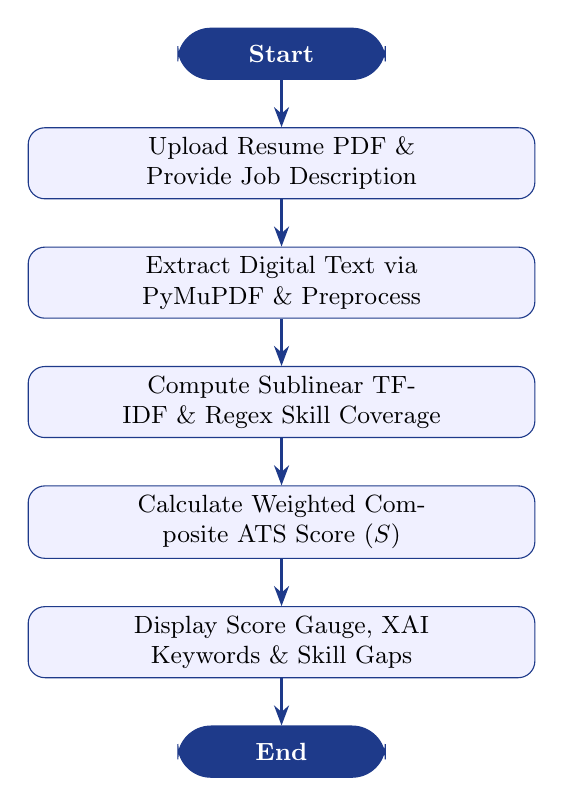
\begin{tikzpicture}[
    node distance=0.6cm,
    stepnode/.style={draw=sggsblue, fill=blue!6, rounded corners=6pt, text width=6.2cm, align=center, minimum height=0.65cm, font=\small},
    terminal/.style={draw=sggsblue, fill=sggsblue, text=white, rounded corners=12pt, text width=2.4cm, align=center, minimum height=0.65cm, font=\small\bfseries},
    arrow/.style={-{Stealth[scale=1.1]}, thick, color=sggsblue}
  ]
    \node[terminal] (start) {Start};
    \node[stepnode, below=of start] (upload) {Upload Resume PDF \& Provide Job Description};
    \node[stepnode, below=of upload] (extract) {Extract Digital Text via PyMuPDF \& Preprocess};
    \node[stepnode, below=of extract] (calc) {Compute Sublinear TF-IDF \& Regex Skill Coverage};
    \node[stepnode, below=of calc] (score) {Calculate Weighted Composite ATS Score ($S$)};
    \node[stepnode, below=of score] (display) {Display Score Gauge, XAI Keywords \& Skill Gaps};
    \node[terminal, below=of display] (end) {End};

    \draw[arrow] (start) -- (upload);
    \draw[arrow] (upload) -- (extract);
    \draw[arrow] (extract) -- (calc);
    \draw[arrow] (calc) -- (score);
    \draw[arrow] (score) -- (display);
    \draw[arrow] (display) -- (end);
  \end{tikzpicture}%
  }
\end{frame}

% ---------------------------------------------------------------------------
% Slide 10: Datasets Used & Technology Stack (New Slide)
% ---------------------------------------------------------------------------
\begin{frame}{Datasets Used \& Technology Stack}
  \small
  \begin{columns}[T]
    \begin{column}{0.50\textwidth}
      \textbf{\large 📊 Primary Benchmark Dataset}
      \begin{block}{Kaggle: Updated Resume Dataset}
        \begin{itemize}
          \item \textbf{Source:} Hosted on Kaggle by Jillani SofTech.
          \item \textbf{Volume:} \textbf{962 genuine resumes} across \textbf{25 job categories}.
          \item \textbf{Domains Included:} Data Science (40), Java (84), DevOps (55), Python (48), Testing (70), Web Design (45), HR (44), Blockchain (40), etc.
          \item \textbf{Role in Project:} Multi-candidate benchmarking, domain filtering, and population score distributions.
        \end{itemize}
      \end{block}
      \textbf{Job Benchmark:} 5 curated industry job postings (Data Scientist, ML Engineer, Full Stack, Analyst, SWE).
    \end{column}

    \begin{column}{0.48\textwidth}
      \textbf{\large 💻 Technology Stack Used}
      \begin{itemize}
        \item \textbf{Python 3.10+:} Core programming runtime.
        \item \textbf{Streamlit:} Frontend UI with 3D floating cards and Light Theme styling.
        \item \textbf{Scikit-Learn:} \texttt{TfidfVectorizer}, sublinear TF scaling, and cosine similarity.
        \item \textbf{PyMuPDF (\texttt{fitz}):} High-speed C-based text extraction from digital PDFs.
        \item \textbf{Pandas \& NumPy:} Vector math and candidate ranking.
        \item \textbf{Plotly:} Interactive ATS gauge, radar, and horizontal ranking charts.
        \item \textbf{Pytest:} 55 automated unit and integration tests.
      \end{itemize}
    \end{column}
  \end{columns}
\end{frame}

% ---------------------------------------------------------------------------
% Slide 11: Experiment Results & Candidate Benchmarking
% ---------------------------------------------------------------------------
\begin{frame}{Experiment Results \& Candidate Benchmarking}
  \small
  \textbf{Controlled Candidate Discrimination Benchmark (Target: Machine Learning Role):}
  \begin{table}[h]
    \centering
    \begin{tabular}{l l c c c}
      \toprule
      \textbf{Candidate Profile} & \textbf{Candidate Background} & \textbf{Cosine Sim} & \textbf{Skill Coverage} & \textbf{Composite Score} \\
      \midrule
      \textbf{Eva Chen} & Senior AI/ML Engineer (PyTorch, MLOps) & 78.4\% & 85.7\% & \textbf{82.1\% (Strong Match)} \\
      \textbf{Carol Smith} & M.Sc. Data Science (Spark, Statistics) & 64.2\% & 71.4\% & \textbf{67.8\% (Good Fit)} \\
      \textbf{Alice Johnson} & B.Tech CS Fresher (Python, EDA, Scikit) & 51.0\% & 57.1\% & \textbf{54.1\% (Moderate Fit)} \\
      \textbf{Bob Martinez} & Full Stack Developer (React, Django) & 32.5\% & 14.3\% & \textbf{23.4\% (Low Relevance)} \\
      \textbf{David Lee} & IT Support / Basic Generalist & 18.2\% & 0.0\% & \textbf{9.1\% (Disqualified)} \\
      \bottomrule
    \end{tabular}
  \end{table}

  \textbf{Performance \& Testing Telemetry:}
  \begin{itemize}
    \item \textbf{Processing Latency:} Under \textbf{25 milliseconds} per resume on standard laptop CPU.
    \item \textbf{Automated Test Suite:} \textbf{55 unit and integration tests passing} (100\% pass rate).
  \end{itemize}
\end{frame}

% ---------------------------------------------------------------------------
% Slide 12: Limitations
% ---------------------------------------------------------------------------
\begin{frame}{Limitations}
  \textbf{Current System Limitations:}
  \begin{itemize}
    \item \textbf{Digital Text Dependency:} System relies on readable digital text streams; image-only scanned PDFs require an Optical Character Recognition (OCR) preprocessor.
    \item \textbf{Lexical Matching vs. Deep Synonyms:} Pure TF-IDF measures exact lexical and bigram overlap. It cannot infer that `"ML Developer"` is identical to `"Machine Learning Engineer"` without explicit aliases.
    \item \textbf{Static Skill Dictionary:} Skill detection is bounded by the predefined technical taxonomy in \texttt{skills.py}.
    \item \textbf{Decision-Support System:} The platform is engineered to assist and augment human recruiter screening, not to make unilateral hiring decisions.
  \end{itemize}
\end{frame}

% ---------------------------------------------------------------------------
% Slide 13: Future Scope
% ---------------------------------------------------------------------------
\begin{frame}{Future Scope}
  \textbf{Planned Architectural Improvements:}
  \begin{itemize}
    \item \textbf{Dense Semantic Embeddings:} Integrate Sentence-BERT (\texttt{all-MiniLM-L6-v2}) to calculate hybrid lexical-semantic cosine similarity and resolve synonyms.
    \item \textbf{OCR Pipeline Integration:} Add Tesseract OCR or PaddleOCR to automatically extract text from scanned, image-only resume PDFs.
    \item \textbf{Dynamic Ontology Expansion:} Use automated web scraping of GitHub/StackOverflow to continually update the technical skill taxonomy.
    \item \textbf{Enterprise HRMS Connectors:} Deploy REST API webhooks for seamless integration with corporate ATS platforms (Workday, Greenhouse, Taleo).
  \end{itemize}
\end{frame}

% ---------------------------------------------------------------------------
% Slide 14: Conclusion
% ---------------------------------------------------------------------------
\begin{frame}{Conclusion}
  \begin{itemize}
    \item Successfully built an automated, objective, and explainable ATS matching system using NLP and Unsupervised Machine Learning.
    \item Formulated a dual-axis composite scoring engine combining contextual text similarity with discrete hard technical skill coverage.
    \item Solved punctuation corruption for programming languages (\texttt{C++}, \texttt{C\#}, \texttt{.NET}) and neutralized keyword-stuffing exploits.
    \item Demonstrated high candidate discrimination accuracy across 962 genuine resumes in the Kaggle dataset in $<25\text{ms}$.
  \end{itemize}

  \vspace{0.2cm}
  \begin{block}{Overall Outcome}
    The ATS Resume Matcher delivers a production-ready, 100\% local, and privacy-preserving platform that replaces opaque black-box scoring with mathematically explainable candidate evaluation.
  \end{block}
\end{frame}

% ---------------------------------------------------------------------------
% Slide 15: References
% ---------------------------------------------------------------------------
\begin{frame}{References}
  \scriptsize
  \begin{enumerate}
    \item \textbf{Singh, I., \& Garg, A. (2024).} \textit{Resume Ranking with TF-IDF, Cosine Similarity and Named Entity Recognition}. IEEE ICDCC, DOI: 10.1109/icdcc62744.2024.10961659.
    \item \textbf{Pendhari, H., Rodricks, S., Patel, M., et al. (2023).} \textit{Resume Screening using Machine Learning}. IEEE ICDSAAI, DOI: 10.1109/icdsaai59313.2023.10452483.
    \item \textbf{Panda, A. R., Kumar, R., Ghosh, A., et al. (2024).} \textit{Optimizing Resume Screening with Machine Learning: An NLP Approach}. IEEE CINE, DOI: 10.1109/cine63708.2024.10881885.
    \item \textbf{Sinha, A. K., Akhtar, M. A. K., \& Kumar, A. (2021).} \textit{Resume Screening Using NLP and Machine Learning: A Systematic Review}. Springer Nature AISC, DOI: 10.1007/978-981-33-4859-2\_21.
    \item \textbf{Salton, G., Wong, A., \& Yang, C. S. (1975).} \textit{A Vector Space Model for Automatic Indexing}. Communications of the ACM, 18(11), 613--620.
    \item \textbf{Kaggle Updated Resume Dataset:} Hosted by Jillani SofTech, \url{https://www.kaggle.com/datasets/jillanisofttech/updated-resume-dataset}.
  \end{enumerate}
\end{frame}

% ---------------------------------------------------------------------------
% Slide 16: Thank You Slide
% ---------------------------------------------------------------------------
\begin{frame}[plain]
  \centering
  \vspace{1.5cm}
  {\Huge \textbf{\textcolor{sggsblue}{Thank You!}}} \\[0.5cm]
  {\large \textbf{Questions \& Discussion Welcome}} \\[1.0cm]

  \begin{block}{Project Repository}
    \centering
    \textbf{GitHub:} \url{https://github.com/aryan9272/MatchMyResume.git}
  \end{block}
\end{frame}

\end{document}
